\chapter{Propuesta}\label{chapter:proposal}
 
    El objetivo de desarrollar un sistema para generar resúmenes de eventos deportivos independiente de la fuente de datos 
planteó distintos retos. El primero de estos fue la necesidad de definir una esquema que abstrajera las características 
generales del conjunto de deportes de enfrentamientos (enfrentamientos dos a dos). Junto con dicho esquema se necesitó 
deifinir una estructura común para la entrada de los datos que permitiera expresar los conocimientos del dominio. Se seleccinó 
una estructura basada en tuplas de cuatro elementos (cuatro-tupla en lo adelante). A parir de esta estructura y en base 
al esquema de definición general se buscó poder determinar esquemas específicos para cada deporte que se fuera a incluir en el 
sistema. Cada uno de estos esquemas específicos son los que se encargan de definir un deporte de forma individualmente dentro del sistema.
    
    La segunda parte del trabajo consistió en construir en base a la propuesta, un esquema y su modelo correspondiente para generar 
resúmenes de partidos de fútbol. Lo mismo se realizó con un deporte de naturaleza diferente como el boxeo.

\section{Propuesta de Esquema General}

    Los deportes se pueden clasificar en la categoría de individuales o colectivos. En los deportes colectivos, las representaciones 
del enfrentamiento ocurren en base a equipos que agrupan a individuos. A su vez en los deportes individuales son dos individuos que se enfrantan.
Esta es la primera diferencia que se extrae en el análisis del conjunto de deportes. Las modalidades analizadas entán representadas en \ref{tab:table_deportes_seleccionados}, 
clasificadas en cuanto a si son individuales o colectivas.

% Please add the following required packages to your document preamble:
% \usepackage{multirow}
\begin{table}[]
    \begin{center}
    \begin{tabular}{|c|c|}
    \hline
    Colectivos                                                                                                                                          & Individuales                                                                                                     \\ \hline
    \multirow{5}{*}{\begin{tabular}[c]{@{}c@{}}Béisbol, Voleibol, \\ Fútbol, Tenis Dobles, \\ Baloncesto, Waterpolo, \\ Balonmano, Hockey\end{tabular}} & \multirow{5}{*}{\begin{tabular}[c]{@{}c@{}}Tenis, Esgrima, \\ Boxeo, Judo,\\ Lucha libre, Taekwondo\end{tabular}} \\
                                                                                                                                                        &                                                                                                                  \\
                                                                                                                                                        &                                                                                                                  \\
                                                                                                                                                        &                                                                                                                  \\
                                                                                                                                                        &                                                                                                                  \\ \hline
    \end{tabular}
    \caption{Deportes analizados}
    \label{tab:table_deportes_seleccionados}
    \end{center}
\end{table}

    De cada uno de estos deportes se analizó:

    \begin{itemize}
        \item Naturaleza de decisión: La mayoría de los deportes se definen como juegos 
        adversariales por acumulación de puntos. La entidad con mayor puntuación gana. Otros como el tenis y el voleibol 
        se definen por cantidad de etapas ganadas (sets), y cada etapa se gana por puntos. A su vez en el boxeo la definición 
        se deriva de votaciones de árbitros.
        \item Posibilidad de empate: Hay deportes como el fútbol que según la competición existe la posibilidad de 
        definirse sin ganadores ni perdedores
        \item Como se dividen los eventos: La mayoría de los eventos se divide por etapas de tiempo
        constante, una excepción es el judo que ocurre de forma continua durante cuatro minutos. 
        \item Alargues de tiempo: La mayoría de los deportes, en caso de no definición en su tiempo reglamentario presentan 
        etapas adicionales en forma punto de oro (ej. judo),  tiempos extras (ej. béisbol, fútbol), tiebreak(desemapte, ej. Voleibol, tenis).
        \item Roles: Dentro de los deportes los participantes ejercen roles, como puede ser su posición en los deportes colectivos. En los deportes 
        individuales estos roles no son tan explícitos.
        \item  Acciones principales: La definición de los eventos ocurre a través de acciones relevantes que ocurren durante el tiempo de juego.
    \end{itemize}

    Del análisis también se extrajeron un conjunto de características que son comunes a los enferntamientos deportivos: la presencia de una sede, 
un público, una fecha. Así mismo, los enfrentamientos normalmente se encuadran dentro de un torneo, y existen distintiones entre categorías lo mismo sea 
de edad, sexo, u de otro tipo (ej. peso).

    A partir del análisis se definió un meta esquema general de tipos de entradas basado en una estructura de 
cuatro-tuplas de conocimiento.

\begin{table}[]
    \begin{center}

\begin{tabular}{|c|c|}
    \hline
    Tipo de Entrada  & Estructura                                                                                                               \\ \hline
    SEDE             & \begin{tabular}[c]{@{}c@{}}(TipoSEDE, \\ Nombre\\ Asistencia\\ Capacidad)\end{tabular}                                   \\ \hline
    TORNEO           & \begin{tabular}[c]{@{}c@{}}(TipoTORNEO\\  Nombre\\ Expresión de Género\\  Expresión de Categoría)\end{tabular}           \\ \hline
    ENFRENTAMIENTO   & \begin{tabular}[c]{@{}c@{}}(TipoENFRENTAMIENTO\\ Entidad\_1\\  Entidad\_2\\  Expresión de Fecha)\end{tabular}            \\ \hline
    ROLENJUEGO       & \begin{tabular}[c]{@{}c@{}}(TipoROLENJUEGO\\  Entidad del Rol\\  Entidad Complementaria\\ Rol Complementario)\end{tabular}   \\ \hline
    RESULTADOPARCIAL & \begin{tabular}[c]{@{}c@{}}(TipoRESULTADOPARCIAL\\ Entidad\\ Indicador de parcial\\ Expresión de puntuación)\end{tabular}    \\ \hline
    RESULTADOFINAL   & \begin{tabular}[c]{@{}c@{}}(TipoRESULTADOFINAL\\ Entidad\\ Expresión de puntuación\\  Descriptor de resultado)\end{tabular}  \\ \hline
    EVENTO           & \begin{tabular}[c]{@{}c@{}}(TipoEVENTO\\  Expresión de Tiempo\\ Entidad Protagonista\\  Entidad Complementaria)\end{tabular} \\ \hline
    \end{tabular}
        
    \end{center}
    \caption{Meta esquema general para definir las entradas de cada deporte}
    \label{tab:esquema_general}
\end{table}

    Cada cuatro-tupla tiene en la primera posición el tipo de entrada. El resto de valores constituyen la base de información. Con cada tipo de entrada 
se encapsula un subconjunto de la información que se muestra común al conjunto de deportes estudiados. 
    A patir del meta esquema general, es posible definir los esquemas específicos de cada deporte, con sus tipos particulares para cada entrada y su forma de interpretar 
cada uno de los valores. Los esquemas de cada deporten tiene que ser capaces de poder expresar la información del mismo para poder a través de ella 
generar textos que describan el evento. A continuación se presenta la definición para dos deportes de naturaleza y estructura muy dispar: el fútbol y 
el boxeo.


\section{Definición y modelo generador para el fútbol}

    Necesario antes de la introducción del modelo es la definición del esquema específico que se utilizó para 
definir y validar las posibles entradas del sistema.

\subsection{Esquema de entrada de datos}

    La experiencia del autor sobre el dominio a tratar así como la consulta del sitio web \textit{whoscored.com} sirvieron para realizar la caracterización del 
fútbol como deporte. Trabajos prervios que también abordaron este deporte para la generación de texto como (~\cite{theune2001data,aires2016automatic,van2017pass}) se tuvieron en cuenta. 
El sitio \textit{whoscored.com} aúna estadísticas y anotaciones de los eventos que ocurren durante un partido de fútbol y dispone de información de miles de encuentros.

A partir de este análisis, se definió es esquema del fútbol como se muestra en \ref{tab:esquema_futbol}

\begin{table}[]
    \begin{center}
        

\begin{tabular}{|c|c|}
    \hline
    Tipo de Entrada  & Valores en el Esquema del Fútbol                                           \\ \hline
    SEDE             & Estadio                                                                    \\ \hline
    TORNEO           & Torneo                                                                     \\ \hline
    ENFRENTAMIENTO   & PartidoPresentacion                                                        \\ \hline
    ROLENJUEGO       & \begin{tabular}[c]{@{}c@{}}Titular\\ Suplente\end{tabular}                 \\ \hline
    RESULTADOPARCIAL & \begin{tabular}[c]{@{}c@{}}Tiempos\\ TiemposExtras\\ Penaltis\end{tabular} \\ \hline
    RESULTADOFINAL   & ResultadoFinal                                                             \\ \hline
    EVENTO &
      \begin{tabular}[c]{@{}c@{}}PaseBueno,PaseFallado,PaseClave,PaseAsistencia,\\ TiroPuerta,TiroNoPuerta,Gol,Atajada,\\ EntradaConExito,EntradaFallada,BloqueoDeDisaparo,\\ Recuperación,FaltaFueraDelArea,ManoFueraDelArea,\\ FaltaDentroDelArea,ManoDentroDelArea,PenaltiCometido,\\ AtajadaPenalti,GolPenalti,TiroPenaltiFuera,TarjetaAmarilla,\\ SegundaTarjetaAmarillaRoja,TarjetaRojaDirecta,\\ GolTiroLibre,Autogol,CobraCorner,Cambio,FueraDeJuego\end{tabular} \\ \hline
    \end{tabular}
    \end{center}   
    \caption{Esquema de definición del fútbol}
    \label{tab:esquema_futbol}
\end{table}

Cada esquemma presenta su especificaciones en cuanto a la intrepretación o la representación de los 
valores por tipo de entrada. Este esquema establece las siguientes:

    \begin{itemize}
        \item Tupla \textbf{SEDE}: Las expresiones de \textit{asistencia} y \textit{capacidad} de no ser vacías deben ser expresiones numéricas (ej. "1200").
        \item Tupla \textbf{TORNEO}: La expresión de \textit{género} debe ser una entre "M" y "F" (masculino, femenino). 
        \item Tupla \textbf{ENFRENTAMIENTO}: Las entidades son los nombres de los equipos que se enfrentan. La expresión de \textit{fecha}, de ser incluida, debe seguir
        el siguiente formato: "AAAA-MM-DD HH:MM" (año-mes-día hora:minutos). Es posible que se provea solo el día o la hora, respetando sus formatos específicos.
        \item Tupla \textbf{ROLENJUEGO}: La entidad de Rol es el jugador, y la entidad complementaria su equipo. El \textit{Rol Complementario} indica la posición que 
        desempeña el jugador en el terreno. Debe ser uno entre: \textit{``POR´´} (portero), \textit{``DEF´´} (defensa), \textit{``CEN´´} (centrocampista) o \textit{``DEL´´} (delantero).
        \item Tupla \textbf{RESULTADOPARCIAL}: La entidad es el equipo al que se refiere, el \textit{indicador de parcial} un valor entre 1 y 5 que se refiere al número de la etapa. Para  
        los \textit{Tiempos} los valores son 1 y 2, para los \textit{TiemposExtra}, 3 y 4, y para \textit{Penaltis}, el 5.
        \item Tupla \textbf{RESULTADOFINAL}: La entidad es el equipo al que se refiere, la \textit{puntuación} es la cantidad de goles anotados por el equipo. El \textit{descriptor de 
        resultado} es uno entre ``V´´ (victria), ``E´´ (empate) , ``D´´ (derrota).
        item Tupla \textbf{EVENTO}  
    \end{itemize}





\begin{figure}[!]
    \begin{center}
        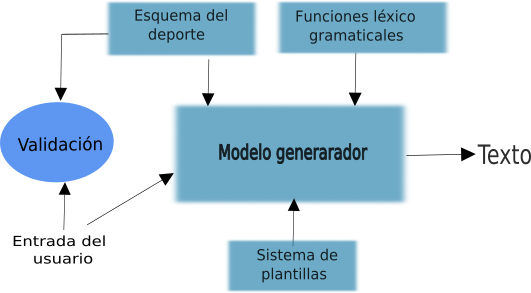
\includegraphics[width=\textwidth]{Graphics/arquitecturaprop2.png}
    \end{center}
    \caption{Arquitectura del modelo propuesto}
    \label{arquitecturadelmodelo}
\end{figure}